\section{Resource-accuracy of retraining configurations}
\label{sec:profiling}


\name relies on accurate estimation of retraining accuracy to decide if the inference model needs to be retrained to cope with data drifts.
% goal
At the $i$-th retraining window, \name's profiler takes in as input a retraining configuration $\gamma\in \Gamma_v$ and returns the estimated accuracy, denoted as $a_v^{(i,\gamma)}$, if \name retrains the model using $\gamma$ now and tests the new model on the remaining portion in the current window.


% natural solution: recent history. not practical for two reasons (1) model is rarely retrained recently, and (2) even it's retrained, the scene will be quite different
A natural strawman is to predict $a_v^{(i,\gamma)}$ using {\em recent history}; \eg a moving-window average over a group of $k$ retraining windows, $a_v^{(i-1,\gamma)},a_v^{(i-2,\gamma)},\dots,a_v^{(i-k,\gamma)}$.
History-based profiling is widely used to optimize machine-learning systems when input data evolve gradually (\eg~\cite{awstream,chameleon}).
However, it may not work well in our setting for two reasons.
First, for the benefits of retraining to outweigh the cost, retraining will only happen intermittently, so the same video is unlikely to have experienced retraining with the same configuration in many of the recent retraining windows.
Second, if the retrain did happen in the last history windows and the model needs to be retrained in the current window, it suggests there has substantial data drift between now and the retraining window when the model was retrained, so the retraining accuracy at that history window may not be indicative to our current window.


% our solution: find history windows that have similar difficulty
Instead, we use history information from more history retraining windows (10s to 100s), but 
% in which the same configuration is used for more times. 
rather than averaging $a_v^{(j,\gamma)}$ over any window $j$, \name uses only the windows whose class distributions are similar to the current window. 
We assume the golden model is running at a low frequency so that it takes negligible resources but still maintain a rough estimate of the distribution of classes in each retraining window.


The insight is that the accuracy of a retrained model depends more on difficulty of the data used to retrain the model. 
For instance, if the training data consist of only a handful of classes, the retrained model can be very high accurate since the data have low complexity.
Otherwise, if the training data include tens of classes, the retrained model will tend to have slightly lower accuracy on each class, due to the inherent capacity/complexity tradeoff of cheap DNN models.
In other words, if two retraining windows are comprised of similar distribution of classes, the retraining accuracies tend to similar. (Of course, there can be other metric of difficulty of the training data than class distribution, but we empirically found class distribution works well in our setting.)
There are other refinements that can be integrated in \name.
For instance, one can try several retraining configurations in parallel on a small subsample of the training data. 
In the case when there is no history window with similar class distribution that used the queried retraining configuration, by default \name will apply the configuration to retrain the model (if there is enough resource).

% some empirical numbers
To show the effectiveness of our idea, Figure~\ref{fig:profiler-error} picks a retraining configuration (retraining last layer of ResNet18) and compares the prediction error of two strategies per Waymo retraining window: running average over recent four history windows (baseline) and average over windows with similar class distributions (\name's profiler).\footnote{Notice that this is an idealized assumption; \name will not have a measured accuracy of the same configuration in all history windows, but the fact that our method based on class distribution similarity uses less windows, so in practice, our prediction can be even more accurate than the baseline.}
To identify retraining windows that have similar class distribution, we group the class distributions into 5 clusters which acount for 70\% of retraining windows.
We see that \name has on average 10\% lower prediction errors (with more reduction on the high percentiles).
We should stress that even if two windows have similar class distributions, it does not mean the retrained model from one window can be re-used in the other due to discrepancies in other aspects (camera lighting, angle, etc).

\begin{figure}[t]
\centering
%\includegraphics[width=0.4\textwidth]{figs/junchen/video-market-new.pdf}
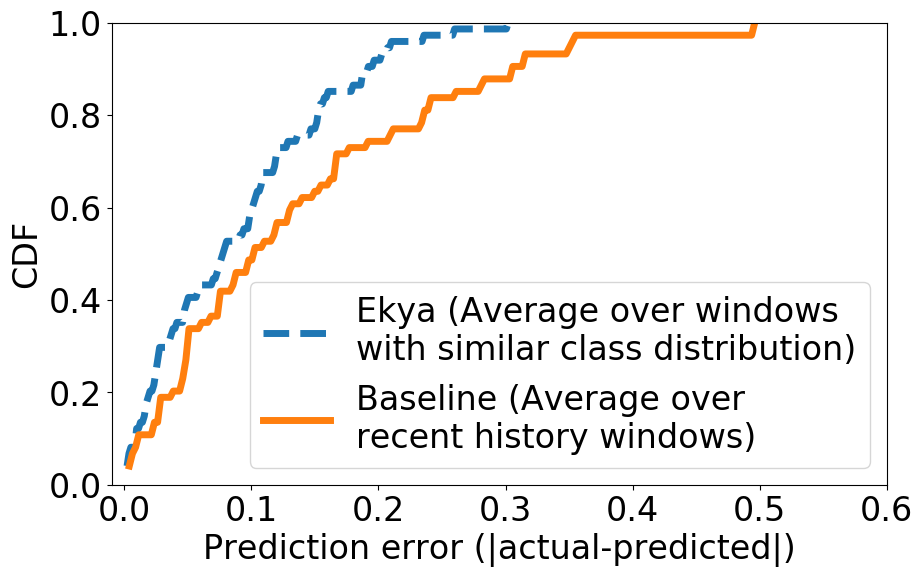
\includegraphics[width=0.3\textwidth]{figures/eval_placeholders/cdf-profiler-error.png}
\vspace{-0.2cm}
\caption{\name's profiler can predict the model accuracy after retraining with less error than the baseline of moving average over recent history windows.
\vspace{-0.2cm}}
\label{fig:profiler-error}
\end{figure}